\documentclass[	DIV=calc,%
							paper=letter,%
							fontsize=12pt%,%
							%twocolumn
                            ]{scrartcl}	 					% KOMA-article class

\usepackage{listings} 
\lstset{language=Matlab} 
\usepackage{lipsum}													% Package to create dummy text
\usepackage[utf8]{inputenc}
\usepackage[spanish]{babel}										% English language/hyphenation
\usepackage[protrusion=true,expansion=true]{microtype}				% Better typography
\usepackage{amsmath,amsfonts,amsthm,mathabx}					% Math packages
\usepackage[pdftex]{graphicx}									% Enable pdflatex
\usepackage[svgnames]{xcolor}									% Enabling colors by their 'svgnames'
\usepackage[hang, small,labelfont=bf,up,textfont=it,up]{caption}	% Custom captions under/above floats
\usepackage{epstopdf}												% Converts .eps to .pdf
\usepackage{subfig}													% Subfigures
\usepackage{booktabs}												% Nicer tables
\usepackage{fix-cm}	
\usepackage{pgfgantt}											% Custom fontsizes
\usepackage{framed}
\newenvironment{digression}[1]{\begin{shaded} \noindent\textbf{\sc {#1}\\} }{ \end{shaded} } % or snugshade
\definecolor{shadecolor}{rgb}{0.98,0.93,0.7}
\usepackage{pgfplots}

%%% Custom sectioning (sectsty package)
\usepackage{sectsty}													% Custom sectioning (see below)
\allsectionsfont{%															% Change font of al section commands
	\usefont{OT1}{phv}{b}{n}%										% bch-b-n: CharterBT-Bold font
	}

\sectionfont{%																% Change font of \section command
	\usefont{OT1}{phv}{b}{n}%										% bch-b-n: CharterBT-Bold font
	}



%%% Headers and footers
\usepackage{fancyhdr}												% Needed to define custom headers/footers
	\pagestyle{fancy}														% Enabling the custom headers/footers
\usepackage{lastpage}	

% Header (empty)
\lhead{}
\chead{}
\rhead{}
% Footer (you may change this to your own needs)
\lfoot{\footnotesize \texttt{Sistemas Electrónicos para Smart Gruids} \textbullet ~2017}
\cfoot{}
\rfoot{\footnotesize p\'agina \thepage\ de \pageref{LastPage}}	% "Page 1 of 2"
\renewcommand{\headrulewidth}{0.0pt}
\renewcommand{\footrulewidth}{0.4pt}
\addto\captionsenglish{\renewcommand{\figurename}{Fig.}}
\addto\captionsenglish{\renewcommand{\tablename}{Tabla}}
\addto\captionsenglish{\renewcommand{\refname}{Bibliograf\'ia}} 


%%% Creating an initial of the very first character of the content
\usepackage{lettrine}
\newcommand{\initial}[1]{%
     \lettrine[lines=3,lhang=0.3,nindent=0em]{
     				\color{DarkGoldenrod}
     				{\textsf{#1}}}{}}



%%% Title, author and date metadata
\usepackage{titling}															% For custom titles

\newcommand{\HorRule}{\color{DarkGoldenrod}%			% Creating a horizontal rule
									  	\rule{\linewidth}{1pt}%
										}

\pretitle{\vspace{-30pt} \begin{flushleft} \HorRule 
				\fontsize{35}{35} \usefont{OT1}{phv}{b}{n} \color{DarkRed} \selectfont 
				}
\title{Algoritmo Hill-Climbing MPPT para la obtención de máxima potencia a la salida un panel solar fotovoltaico }					% Title of your article goes here
\posttitle{\par\end{flushleft}\vskip 0.5em}

\preauthor{\begin{flushleft}
					\large \lineskip 0.5em \usefont{OT1}{phv}{b}{sl} \color{DarkRed}}
\author{Juan Moreno Nadales }											% Author name goes here
\postauthor{\footnotesize \usefont{OT1}{phv}{m}{sl} \color{Black} 
					 								% Institution of author
					\par\end{flushleft}\HorRule}

\date{}																				% No date



%%% Begin document
\begin{document}
\maketitle
\thispagestyle{fancy} 			% Enabling the custom headers/footers for the first page 
% The first character should be within \initial{}
\initial{S}\textbf{e desea llevar a cabo la implementación de un algoritmo MPPT de tipo Hill-Climbing para la obtención de máxima potencia a la salida de un panel fotovoltaico conectado a red}\\\\


\newpage

\tableofcontents
\listoffigures
\newpage


\section{Introducción}

Uno de los retos a los que se enfrenta la sociedad actual es la integración de las fuentes de energía renovables como base de suministro de potencia de la red. En este ámbito, es común encontrar grandes instalaciones y explotaciones de energías renovables gestionadas por grupos empresariales, como pueden ser los grandes parques eólicos, o los campos de paneles solares térmicos o fotovoltáicos. En contrapartida con este tipo de generación de energía a gran escala, surge la opción de la generación de energía en el ámbito doméstico, bien con fines de autoconsumo o con el objetivo de suministrar potencia a la red a cambio de una serie de retribuciones económicas.

\hfill

En esta práctica analizamos una de estas alternativas a escala doméstica, consistente en un panel fotovoltáico como fuente de alimentación conectado a red a través de una doble etapa de conversión $dc/dc$ y $dc/ac$.

\hfill

Dicho convertidor de doble estará formado en primer lugar por un convertidor $dc/dc$ tipo $flyback$ que cumplirá una doble función. En primer lugar, elevará la tensión suministrada por el panel antes de su entrada al inversor conectado a red. Además de esta función, y debido a la normativa actual que obliga al aislamiento de la fuente generadora de la red, la elección de un convertidor tipo $flyback$ se justifica debido a que mediante la utilización del transformador inherente al convertidor podemos llevar a cabo dicha labor de aislamiento sin necesidad de introducir una nueva etapa.

\hfill

Junto con la estructura del convertidor, el elemento central de la práctica es la implementación de un algoritmo tipo $MPPT$.La familia de algoritmos $MPPT$, siglas de $Maximum Power Point Tracking$, tienen como misión principal, tal y como se detallará y explicará más adelante, conseguir que la fuente de generación de continua, en nuestro caso, el panel fotovoltáico, suministre a su salida el máximo nivel de potencia alcanzable bajo unas determinadas condiciones ambientales. 

\newpage

\section{Algoritmos MPPT}

\subsection{Concepto de MPPT}

La potencia suministrada a la salida de un panel solar, depende fundamentalmente de dos factores, la temperatura ambiental, y el nivel de radiación solar recibida por el panel. Esta última variable, depende a su vez de otra serie de factores, como pueden ser la orientación de los paneles, las condiciones atmosféricas del momento, o incluso la época del año, que está directamente relacionada con la distancia de la tierra al sol. Se muestra a continuación una gráfica que muestra 

\hfill

\begin{figure}[h]
\centering
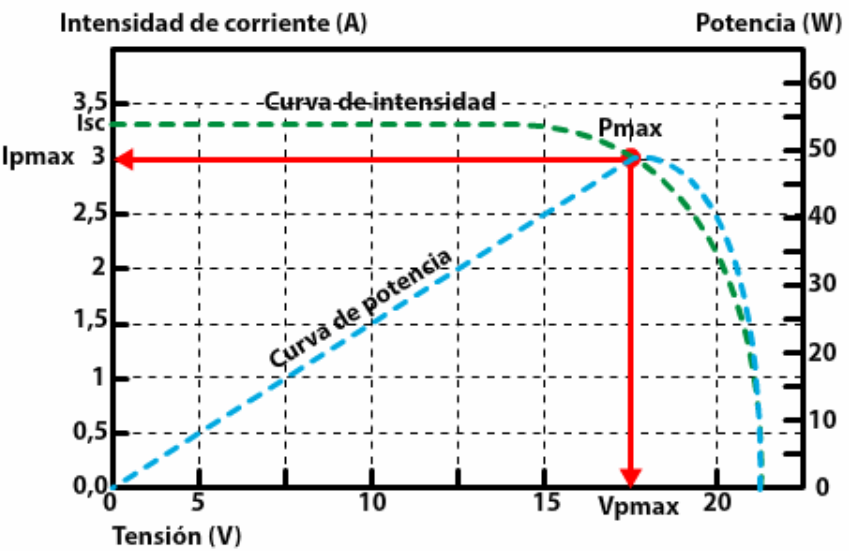
\includegraphics[scale=0.5]{img_mpp}
\caption{Curva de potencia a la salida del panel}
\end{figure}

Como se puede observar en la figura anterior, existen un punto de voltaje y tensión para el cual la potencia obtenida es máxima. El problema surge debido a que un cambio en los condicionantes explicados anteriormente producen a su vez un cambio en la curva $corriente-tension$ y, por lo tanto, un desplazamiento del punto de máximo voltaje.

\hfill
\

Es aquí donde entra en juego el papel de los algoritmos de tipo $MPPT$, cuya labor en todo momento es seguir dicho punto de y asegurar que el panel está suministrando la máxima potencia posible bajos  condiciones ambientales que se den en cada momento.

\hfill
\

\subsection{Hill-Climbing MPPT}

\hfill
\

Dentro de la familia de técnicas $MPPT$ son numerosas las alternativas que se han desarrollado para llevar a cabo el proceso de seguimiento del punto de máxima potencia. Una de las más comunes, es la analizada en esta práctica y conocida como $Hill-Climbing$. Esté algoritmo funciona de la siguiente manera.

\hfill
\

 En todo momento se lleva a cabo una medición de la tensión y la corriente a la salida del penal solar, lo cual nos permite calcular la potencia suministrada por el panel. Una vez calculada la potencia actual, somo capaces de comparar esta con la potencia en el instante anterior, sabiendo así se esta ha incrementado o disminuido y, por lo tanto, la dirección hacia la cual se ha desplazado el punto de máxima potencia. Una vez conocedores de la variación de potencia, hemos de saber si esta variación se ha producido debido a un aumento o disminución del voltaje.
 
 \hfill
 \
 
  En el caso, por ejemplo, de que la potencia haya aumentado y y a su vez se haya producido un aumento de voltaje, ello significaría que podemos desplazar a la derecha el el punto de trabajo, es decir, hemos de aumentar la tensión de referencia de control del convertidor a la salida del panel, ya que de otra forma estaríamos aprovechando menos potencia que la que realmente podemos obtener. Por el contrario, si el aumento de potencia se hubiese producido debido a una disminución de voltaje, ello significaría que el punto de máximo aprovechamiento se encuentra a a la izquierda del punto anterior, lo cual indica que hemos de disminuir el voltaje de trabajo y, por lo tanto, el voltaje de referencia del convertidor.


\newpage

Se muestra a continuación un diagrama $ASM$ del algoritmo.

\hfill
\

\begin{figure}[h]
\centering
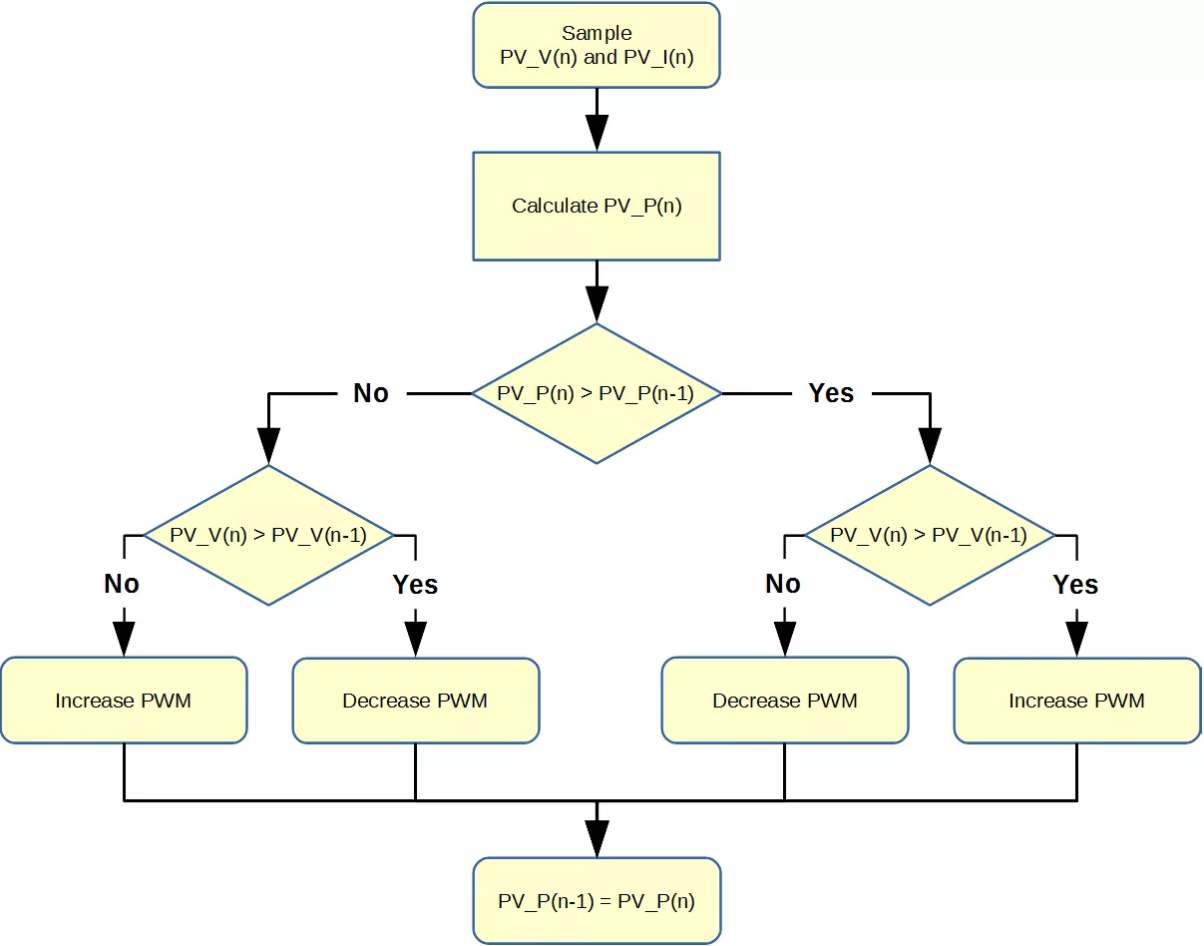
\includegraphics[scale=0.55]{mp2}
\caption{Diagrama ASM del algoritmo $Hill-Climbing$}
\end{figure}

\hfill
\

La implementación de este algoritmo ha sido llevada a cabo en esta práctica en código Matlab, haciendo uso de un archivo de función al cual llamamos desde el esquemático del circuito en Simulink. Se muestra a continuación del código de dciho algoritmo.

\newpage

\begin{lstlisting}[frame=single]  % Inicia el bloque de código
 function sys = mdlOutputs(t,x,u)
% VARIABLES GLOVALES

global Vpv_anterior;
global Ipv_anterior;
global Ppv_anterior;
global Vref;

% ENTRADAS

Vpv=u(1);
Ipv=u(2);

% POTENCIA

Ppv= Vpv*Ipv;

% ALGORITMO MPPT
 
if (Ppv-Ppv_anterior)~=0
    if (Ppv-Ppv_anterior)>0
        if Vpv-Vpv_anterior>0
            Vref=Vref+1;
        else 
            Vref=Vref-1;
        end
    else
        if Vpv-Vpv_anterior>0
            Vref=Vref-1;
        else 
            Vref=Vref+1;
        end
    end
end


\end{lstlisting}

\newpage

\section{Esquema del Circuito}

A continuación veremos todas y cada una de las partes de las que se compone el convertidor diseñado, analizando su comportamiento individual para después llevar acabo la integración total del sistema.

\subsection{Convertidor Flyback y algoritmo MPPT}

El primer paso en la realización de nuestro sistema es llevar a cabo la implementación del convertidor $flyback$ situado a la salida del panel para llevar a cabo la adaptación del nivel de tensión en continua. El objetivo principal no es obtener un determinado nivel a la salida de esta etapa sino, forzando a que la tensión a la salida tome un valor determinando colocando una fuente de alimentación de continua, observar que el algoritmo $MPPT$ prviemente diseñado funciona adecuadamente.

\begin{figure}[h]
\centering
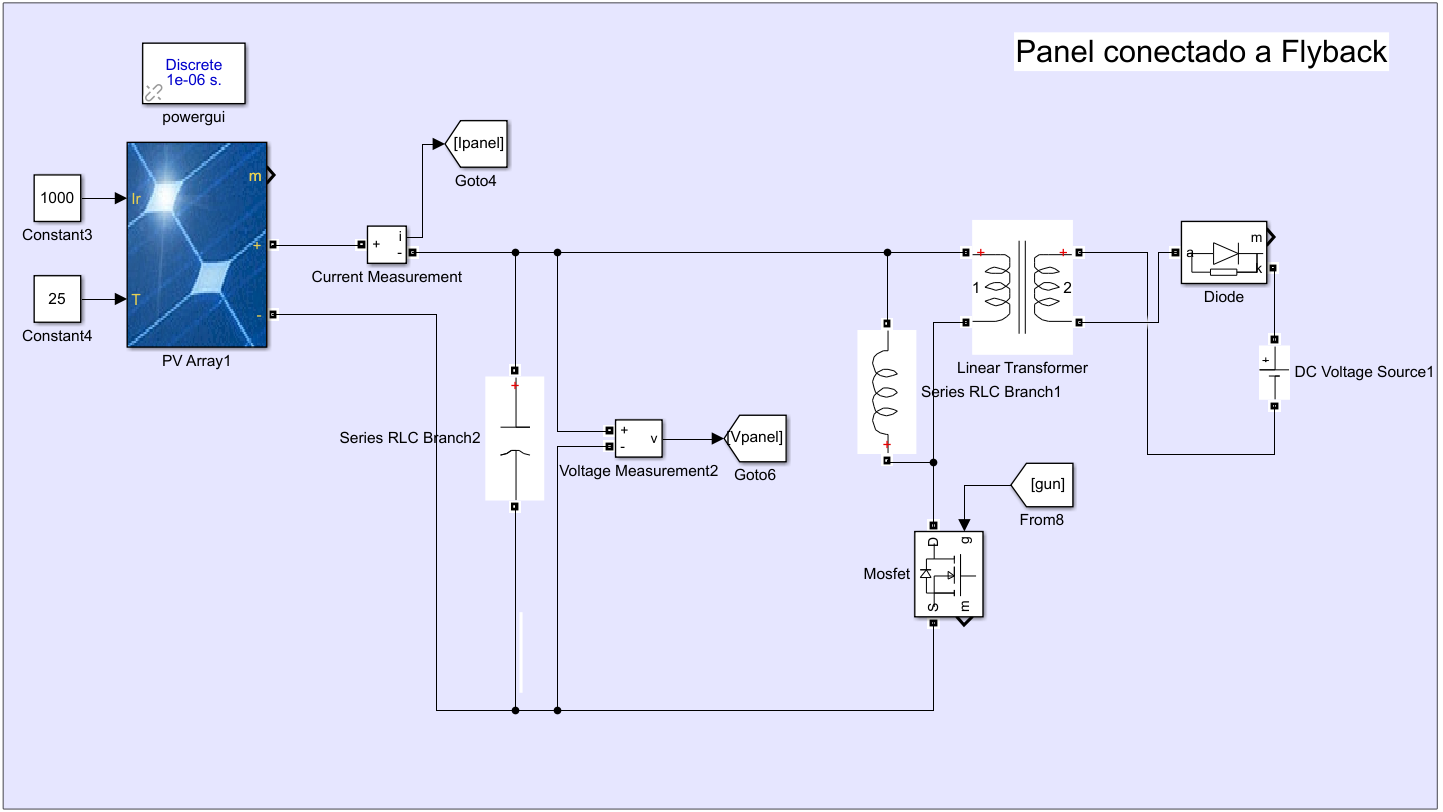
\includegraphics[scale=0.5]{cir_fly}
\caption{Convertidor Flyback}
\end{figure}

\newpage

La figura (3) muestra una imagen del panel conectado al convertidor $flyback$. Para que el sistema funcione, hemos de generar la adecuada señal de control de disparo del transistor que gobierna el convertidor. Para ello se utiliza una modulación PWM la cual se genera mediante la comparación de una señal triangular y la señal de error fruto de la diferencia entre el valor de la tensión e un determinado momento y la tensión de referencia de salida del algoritmo $MPPT$. A continuación de muestran en el esquema de control así como la señal de referencia de salida del algoritmo.

\hfill
\

\begin{figure}[h]
\centering
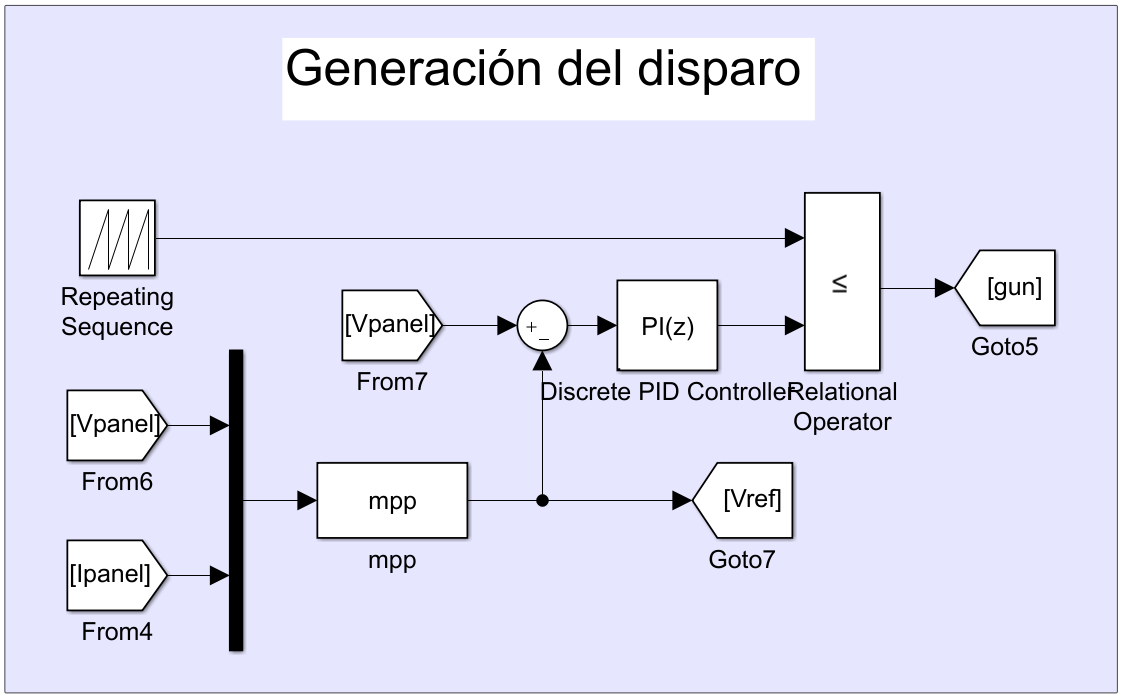
\includegraphics[scale=0.5]{confly}

\hfill
\

\caption{Circuito generador de la señal PWM}
\end{figure}

El objetivo principal de la aplicación de los algoritmos tipo $MPPT$ es la de seguir el punto de máxima potencia en sistemas de generación de energía en los cuales distintos factores ambientales. En nuestro caso estos valores están impuestos y no varían, por lo tanto la señal a la salida del panel se mantendrá siempre dentro de unos determinados valores .A continuación se muestra la figura en la que se ve como la señal a la salida del convertidor sigue  ala señal de referencia  después de un pequeño transitorio.

\newpage

\begin{figure}[h]
\centering
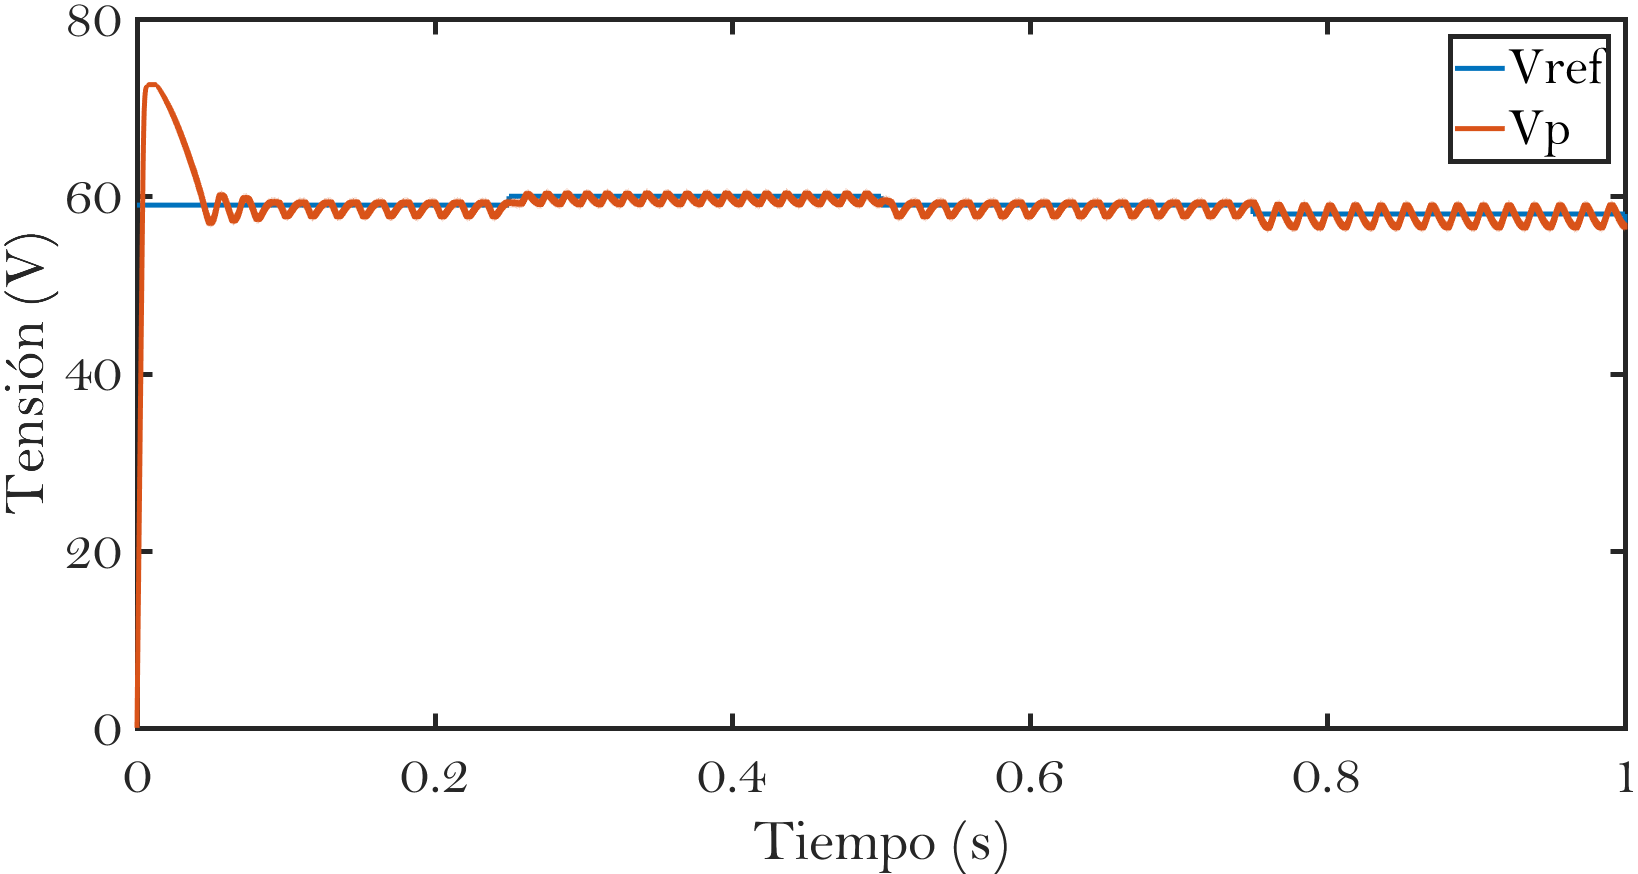
\includegraphics[scale=0.4]{img_1}
\caption{Señal de referencia y señal de tensión a la salida del panel}
\end{figure}


\subsection{Inversor }

\hfill
\

Una vez que hemos comprobado que nuestro algoritmo $MPPT$ funciona adecuadamente, el siguiente paso es diseñar el convertidor inversor que transformará la tensión en continua a la salida del $flyback$ en tensión alterna de red. Inicialmente, y para garantizar que el diseño del convertidor inversor es el correcto, se conectará la entrada del convertidor a una fuente de tensión constante. Para el control de este convertidor se ha decido utilizar momentáneamente  una modulación $PWM$ mediante la comparación de una señal sinusoidal de referencia y una señal triangular, antes de proceder a realizar el control en lazo de tensión y lazo de corriente, tal y como se hará en el siguiente apartado. Se muestran a continuación la imagen del circuito inversor así como su señal de salida con una tensión de entrada de 450 $VDC$ y carga $RL$.

\newpage

\begin{figure}[h]
\centering
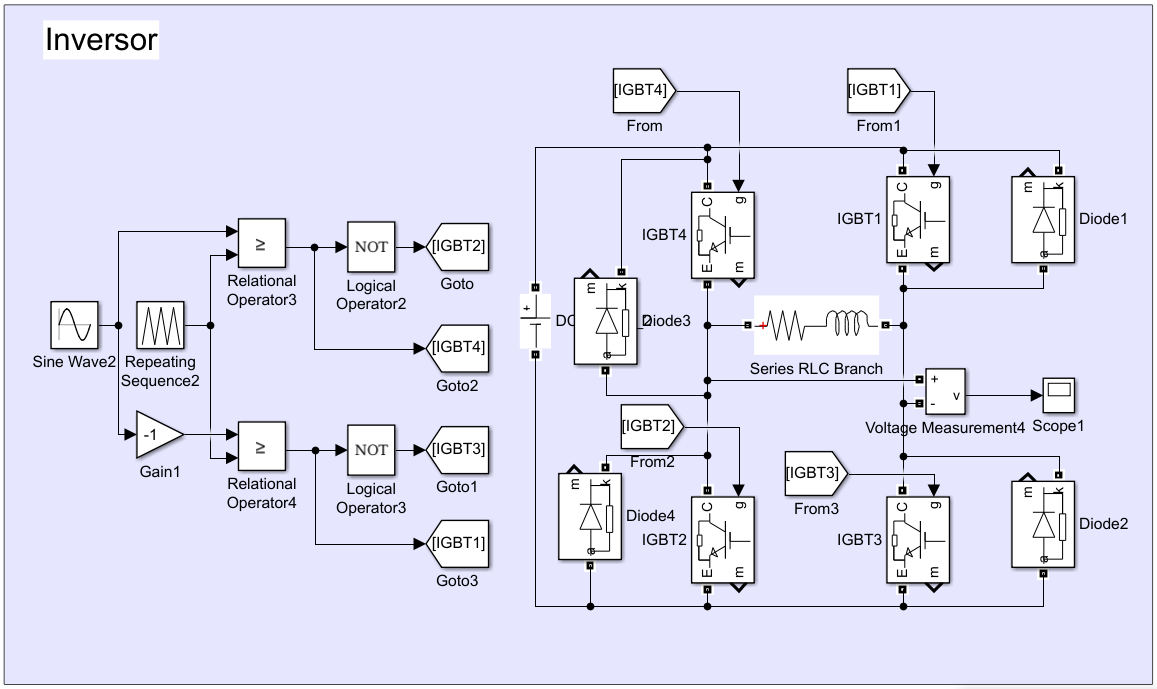
\includegraphics[scale=0.4]{inv_fly}
\caption{Esquema del inversor}

\hfill
\

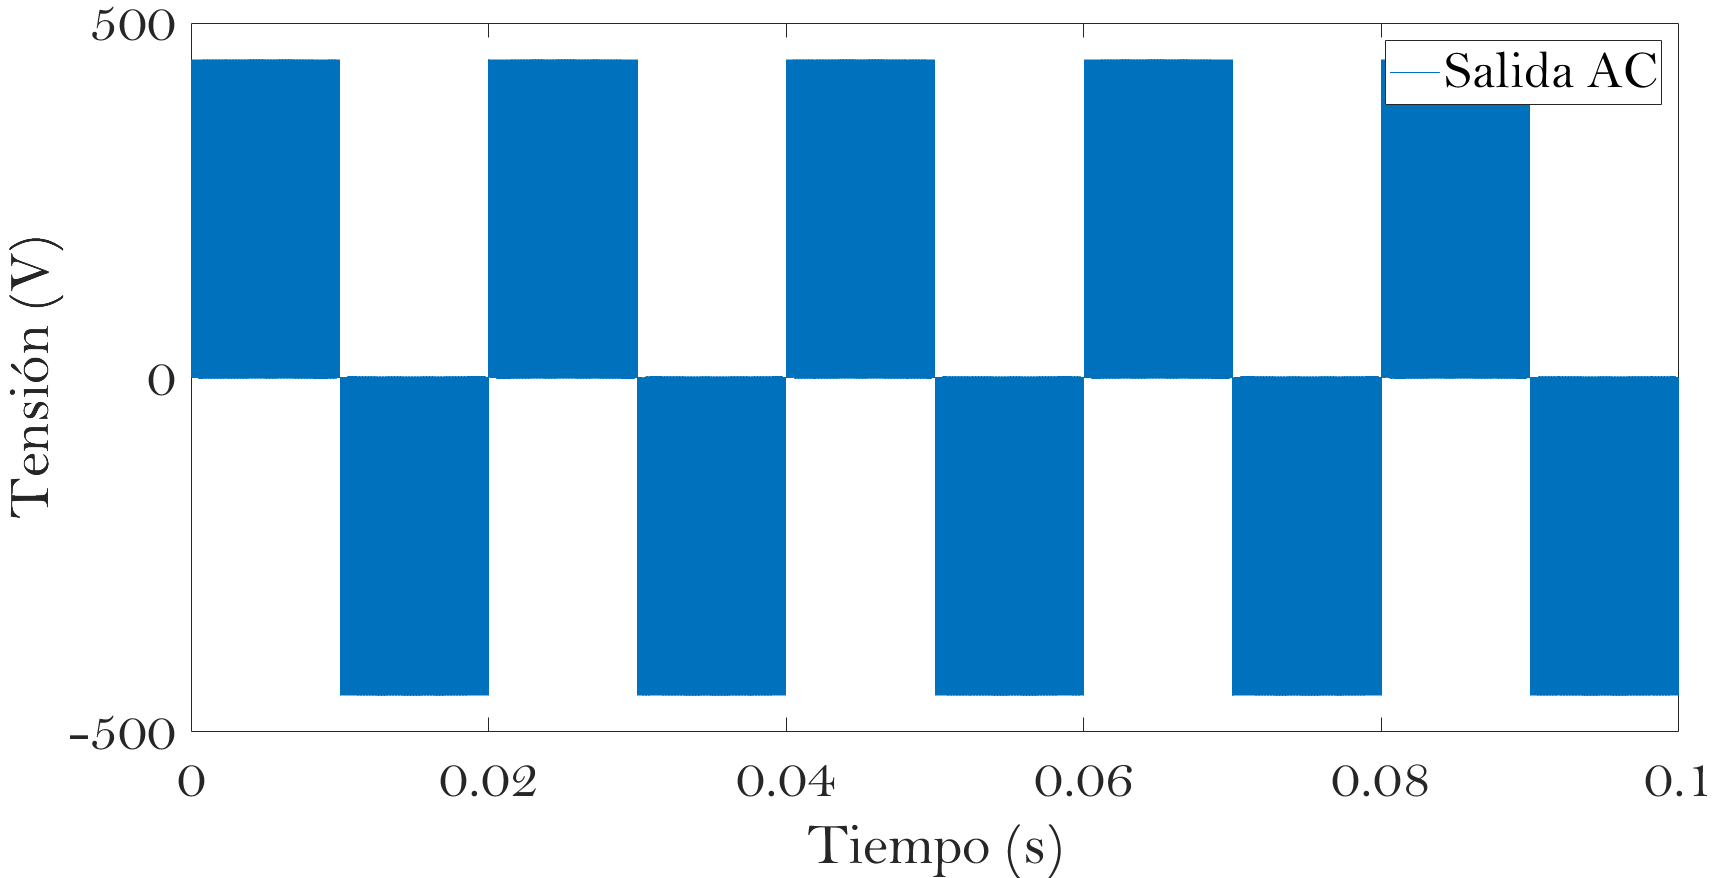
\includegraphics[scale=0.3]{salida}
\caption{Señal de salida del inversor}
\end{figure}

\newpage

\subsection{Inversor conectado a red}

\hfill

Una vez que se han llevado a cabo las tres partes fundamentales de la práctica, a saber, el diseño del convertidor $flyback$, la aplicación del algoritmo $MPPT$, y el diseño del convertidor inversor, nos queda únicamente llevar a cabo la integración de todas las partes del sistema y realizar la conexión de nuestro convertidor a red. Para ello, se eliminarán las fuentes de tensión continua situadas a la salida de la primera etapa y entrada de la segunda y serán sustituidas por un condensador a modo de $DC-Link$ que actuará como fuente de alimentación del inversor conectado a red. Además, con el objetivo de simular el comportamiento de la red, se ha situado a la salida del convertidor inversor una fuente de alimentación en alterna unida a una inductancia de línea.

\hfill
\

Para llevar a cabo el control de los transistores que gobiernan el inversor, se ha llevado a cabo la implementación de un doble lazo cerrado. Por un lado, se compara la tensión $V_{dc}$ real a la salida del convertidor flyback con la tensión deseada, en este caso, de 450 VDC. La señal de error resultante es conducida hacia in controlador tipo PI. Esto garantizará que la tensión en el condensador de enlace se mantenga constante, lo cual no sólo producirá la mejora de  la señal a la salida del convertidor y por tanto su menor componente armónica, sino que además, debido a que la la energía almacenada en un condensador es proporcional a la variación de voltaje en sus bornes, conseguiremos que toda esta energía sea vertida sobre la red y no quede almacenada en el enlace. Seguidamente, se realiza el lazo en corriente, en el cual calculamos el error comparando la corriente deseada obtenida en la etapa anterior con la corriente actual a la salida del sistema. Nuevamente, calculamos la señal de control mediante el uso de un controlado PI que tiene como entrada dicha señal de error. La señal de salida del este bloque PI, correctamente normalizada dividiéndola entre el nivel de tensión deseado, será comparada con una señal triangula, con lo cual obtendremos las señales de disparo de los distintos transistores. Se muestra a continuación una imagen del circuito final así como la tensión a la salida del convertidor.

\newpage

\begin{figure}[h]
\centering

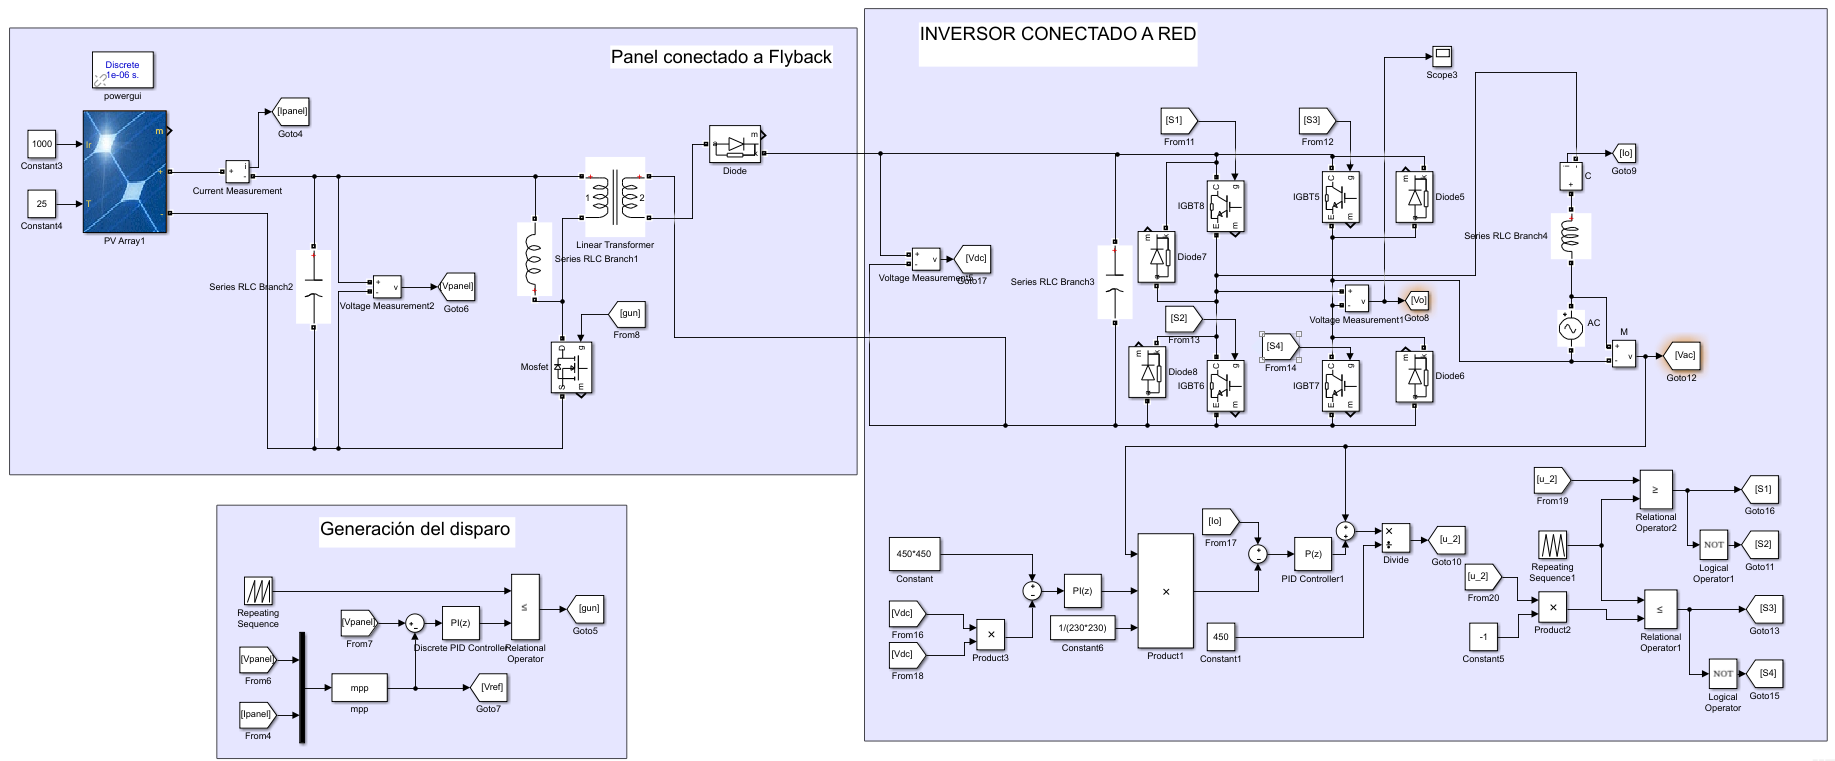
\includegraphics[scale=0.4]{cir_final}
\caption{Esquema completo}

\hfill
\

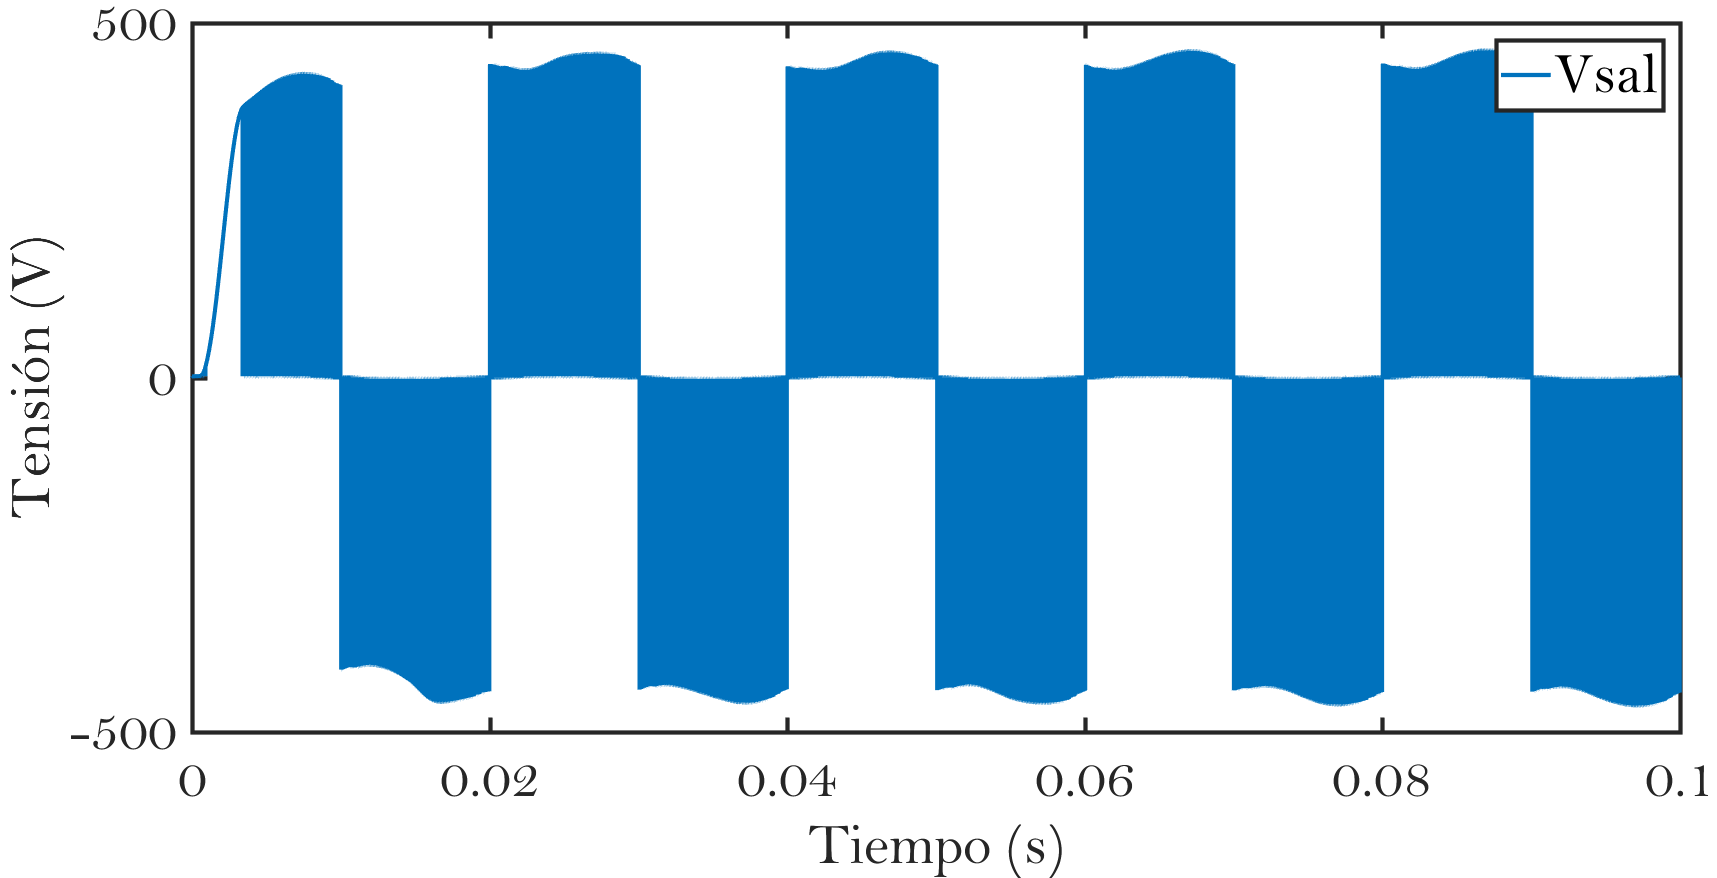
\includegraphics[scale=0.35]{v_fin}
\caption{Señal de salida del inversor}
\end{figure}
\end{document}
\end{document}

